\section{Kiến trúc hệ thống}
Hệ thống được thiết kế với hai module với chức năng của từng module được mô tả dưới đây:
\begin{itemize}
    \item \textbf{Module thu thập dữ liệu cử chỉ:} Đầu vào của khối này là dữ liệu cử chỉ được thu thạp từ các cảm biến flex sensor và cảm biến gyroscope. Dẽ liệu sau khi thu thập sẽ được đóng gói và gửi về module nhận dạng cử chỉ.
    \item \textbf{Module nhận dạng cử chỉ} Dữ liệu được gửi về từ module thu thập sẽ được xử lý, phân loại và đình hình lại dữ liệu để đưa vào mô hình học máy. Đầu ra của mô hình học máy sẽ là kết quả dự đoán cử chỉ dưới dạng văn bản và sẽ được chuyển đổi thành giọng nói qua khối Text-to-speech.
    \item \textbf{Module chuyển văn bản thành giọng nói}: Khi nhận được output đầu ra, module này có chức năng chuyển đầu ra từ dạng one-hot-code output sang dạng văn bản, từ văn bản đó sử dụng thư viện pyttsx3 để phát ra âm thanh như mong muốn đã được cấu hình trước đó trong file config.
\end{itemize}
\begin{figure}[H]
    \centering
    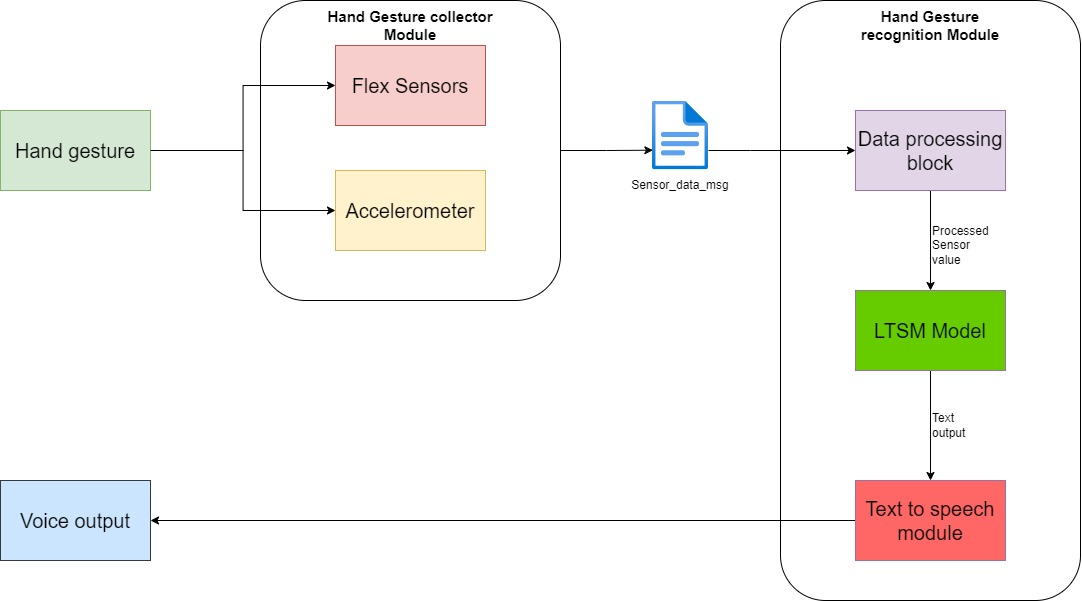
\includegraphics[width=\textwidth,height=\textheight,keepaspectratio]{Images/Theoretical basis/FlexArchitecture.jpg}
    \caption{Kiến trúc tổng quan của hệ thống}
    \label{fig:enter-label}
\end{figure}
\textbf{Mô tả luồng dữ liệu}
\begin{enumerate}
    \item \textbf{Hand Gesture} (Cử chỉ tay):
    \begin{itemize}
        \item Cử chỉ tay là đầu vào của hệ thống
        \item Các cảm biến uốn cong và gia tốc kế trong mô-đun thu thập cử chỉ tay sẽ ghi nhận và gửi dữ liệu này đến khối xử lý dữ liệu
    \end{itemize}

    \item \textbf{Sensor Data Message} (Thông điệp dữ liệu cảm biến):
    \begin{itemize}
        \item Dữ liệu từ cảm biến được đóng gói thành thông điệp và truyền tới mô-đun nhận diện cử chỉ tay
    \end{itemize}

    \item \textbf{Processed Sensor Value} (Giá trị cảm biến đã xử lý):
    \begin{itemize}
        \item Dữ liệu cảm biến được xử lý trong khối xử lý dữ liệu và các đặc trưng được trích xuất
    \end{itemize}

    \item \textbf{Text Output} (Đầu ra văn bản):
    \begin{itemize}
        \item Mô hình học máy dự đoán cử chỉ tay và chuyển đổi nó thành văn bản
    \end{itemize}

    \item \textbf{Voice Output} (Đầu ra giọng nói):
    \begin{itemize}
        \item Văn bản từ mô hình LSTM được chuyển đổi thành giọng nói và phát ra ngoài thông qua mô-đun chuyển văn bản thành giọng nói
    \end{itemize}
\end{enumerate}


Hệ thống này bao gồm hai mô-đun chính và một module phụ: một mô-đun thu thập cử chỉ tay, một mô-đun nhận diện cử chỉ tay và module phát âm thanh. Mô-đun thu thập cử chỉ tay sử dụng các cảm biến uốn cong và gia tốc kế để ghi nhận dữ liệu cử chỉ tay, sau đó truyền dữ liệu này đến mô-đun nhận diện cử chỉ tay. Tại đây, dữ liệu cảm biến được xử lý và đưa vào mô hình học máy để dự đoán cử chỉ tay dưới dạng văn bản. Cuối cùng, văn bản này được chuyển đổi thành giọng nói dựa trên module phát âm thanh


\subsection{Module thu thập dữ liệu cử chỉ}
\begin{figure}[H]
    \centering
    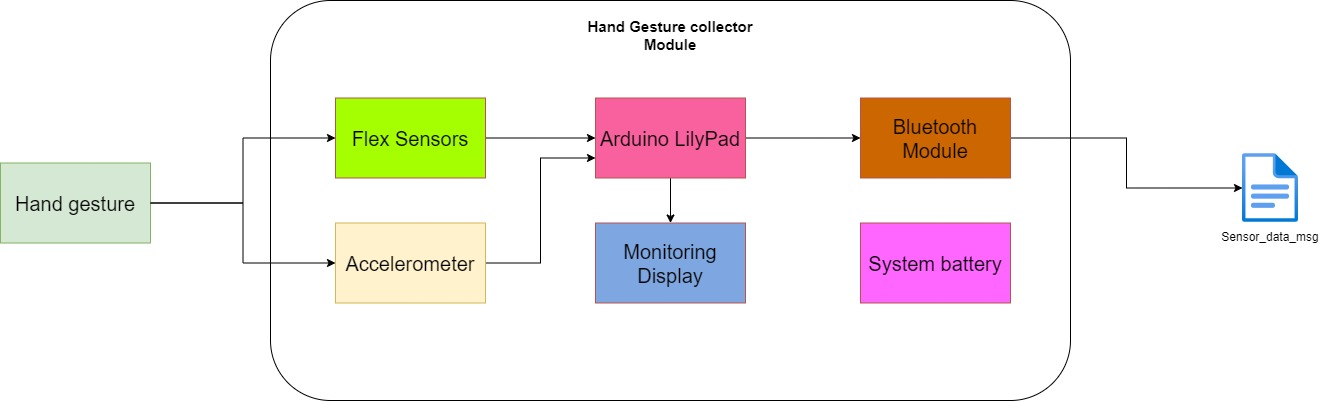
\includegraphics[width=\textwidth,height=\textheight,keepaspectratio]{Images/Theoretical basis/HandGestureCollector.jpg}
    \caption{Kiến trúc module thu thập dữ liệu cử chỉ}
    \label{fig:enter-label}
\end{figure}

Sơ đồ mô tả một hệ thống thu thập cử chỉ tay, gồm các thành phần sau:
\begin{itemize}
\item Hand gesture (Cử chỉ tay): Đây là đầu vào của hệ thống, là các cử chỉ tay cần được nhận diện.
\item Flex Sensors (Cảm biến uốn cong): Nhận tín hiệu từ cử chỉ tay và chuyển tiếp đến Arduino LilyPad.
\item Gyroscope (Cảm biến góc quay): Cũng nhận tín hiệu từ cử chỉ tay và chuyển tiếp đến Arduino LilyPad.
\item Arduino LilyPad: Xử lý dữ liệu nhận được từ Flex Sensors và Gyroscope. Sau đó, chuyển tiếp dữ liệu này đến các thành phần khác.
\item Bluetooth Module (Mô-đun Bluetooth): Truyền dữ liệu từ Arduino LilyPad tới file data
\end{itemize}


Dữ liệu được thu thập từ cử chỉ tay sẽ được xử lý và truyền đi qua mô-đun Bluetooth, sau đó lưu vào file data
\subsection{Module nhận dạng cử chỉ}
\begin{figure}[H]
   \centering
   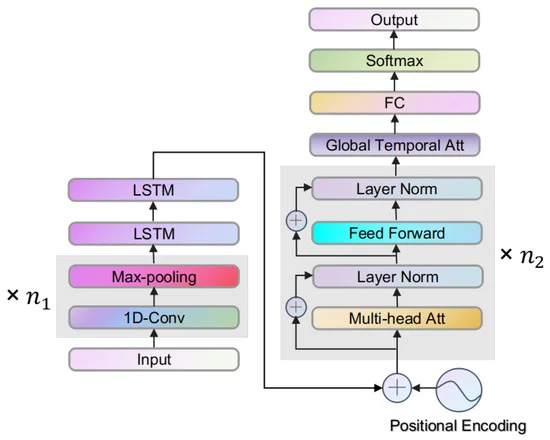
\includegraphics[width=0.8\linewidth]{Images/Architecture/SADeepConv.png}
   \caption{Mô hình mới}
   \label{fig:new-model}
\end{figure}


Để cải thiện độ chính xác của việc nhận dạng cử chỉ, nhóm đã thử nghiệm một mô hình áp dụng cơ chế \textit{self-attention} vào mô hình DeepConvLSTM để thiết lập nên mô hình deep convolutional LSTM dựa trên \textit{self-attention}, gọi tắt là mô hình SADeepConvLSTM. Trên thực tế, cơ chế \textit{self-attention} cho phép mô hình nắm bắt thông tin ngữ cảnh quan trọng trong chuỗi và mối quan hệ quan trọng giữa các đặc trưng của các bước thời gian khác nhau.

Trong hình biểu thị cấu trúc của SADeepConvLSTM mà nhóm đã sử dụng. Nửa bên trái của cấu trúc tuân theo mô hình DeepConvLSTM với các lớp \textit{max pooling}, trong khi nửa bên phải là cấu trúc liên quan đến cơ chế \textit{self-attention}. 


\subsection{Module phát âm thanh}
\begin{figure}[H]
    \centering
    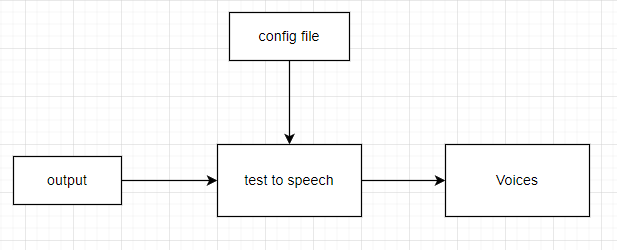
\includegraphics[width=\textwidth,height=\textheight,keepaspectratio]{Images/Theoretical basis/test2speech.png}
    \caption{Kiến trúc module chuyển đầu ra dự đoán thành giọng nói}
    \label{fig:enter-label}
\end{figure}


\subsubsection{Thư viện \texttt{pyttsx3}}

Thư viện \texttt{pyttsx3} trong Python giúp chuyển đổi văn bản thành giọng nói một cách dễ dàng. Nó hoạt động trên nhiều hệ điều hành khác nhau và cho phép người dùng tùy chỉnh giọng đọc, tốc độ nói, ...  Nhờ thiết kế đơn giản và dễ sử dụng, \texttt{pyttsx3} là một công cụ hữu ích để tích hợp chức năng đọc văn bản vào các ứng dụng Python.

\subsubsection{Ứng dụng trong module phát âm thanh}

Module phát âm thanh sử dụng thư viện \texttt{pyttsx3} để "nói" ra kết quả dự đoán hành động. Cụ thể, khi hệ thống nhận dạng được một hành động, nó sẽ tra cứu trong một file cấu hình ("config") để tìm đoạn âm thanh tương ứng với hành động đó. File cấu hình này chứa danh sách các hành động và vị trí của file âm thanh tương ứng với mỗi hành động. Sau đó, module phát âm thanh sẽ sử dụng \texttt{pyttsx3} để phát ra file âm thanh đó.

\subsubsubsection{Ví dụ}

Giả sử hệ thống nhận dạng được hành động "nhảy". Module phát âm thanh sẽ tra cứu trong file cấu hình và tìm thấy file âm thanh tương ứng với hành động "nhảy" (ví dụ: "nhay.mp3"). Sau đó, \texttt{pyttsx3} sẽ được sử dụng để phát file "nhay.mp3".
 

